\chapter{SPECTRE attacks}
	\index{Spectre}In questo capitolo verrà presentato \emph{SPECTRE}\cite{kocher2018spectre}, un tipo di attacco molto recente che sfrutta una vulnerabilità presente nella maggior parte dei processori moderni (Intel, AMD e ARM) e per il quale, al momento, non esistono contromisure.
	
	La vulnerabilità che viene sfruttata da questo tipo di attacco è la cosiddetta \emph{esecuzione speculativa}.
	
	\section{Esecuzione speculativa}
		\index{Esecuzione speculativa}L'esecuzione speculativa è una tecnica utilizzata dai processori per migliorare le prestazioni che consiste nel cercare di "indovinare" il risultato di un branch per eseguire preventivamente alcune istruzioni.
		
		Supponiamo ad esempio che l'esecuzione del programma dipenda da un controllo su di un valore non presente in cache che quindi deve essere recuperato dalla memoria principale. Questo può portare ad un attesa di svariate centinaia di cicli clock prima che questo valore sia disponibile. Invece di aspettare tutto questo tempo inutilmente, il processore cerca di indovinare il risultato del controllo, salva lo stato attuale dei suoi registri, e procede ad eseguire speculativamente il ramo del branch che ritiene più plausibile. Quando poi arriverà il valore effettivo dalla memoria, il controllo verrà effettivamente effettuato. Se il risultato è quello aspettato, si procede con la computazione e saranno stati risparmiati tutti quei cicli di clock che sarebbero stati persi nell'attesa. Se la scelta si rivela sbagliata, il processore scarta tutti i risultati dell'esecuzione speculativa, si riporta allo stato che si era salvato precedentemente ed esegue l'altro ramo del branch.
		
		Questa ottimizzazione sembra perfetta in quanto in caso di successo, si risparmiano molti cicli di clock mentre in caso di insuccesso il risultato è paragonabile a quello che avremmo ottenuto aspettando il dato senza eseguire alcuna istruzione.
		
		Il responsabile di questa scelta è una piccola unità all'interno del processore chiamata \ac{BP}.
		
		\subsection{Branch predictor}
			\index{Branch Predictor}Esistono svariati tipi di branch predictor; andiamo a vedere come funziona uno dei più semplici, il \emph{one-level branch predictor} a 2 bit.
			
			\begin{figure}
				\begin{center}
					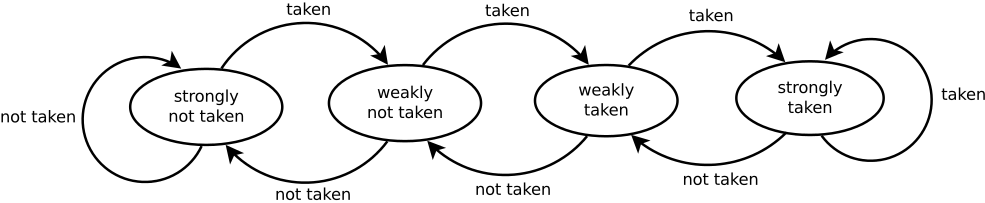
\includegraphics[scale=.35]{bp2bit}
					\caption{Automa di predizione di un one-level branch predictor a 2 bit}
					\label{fig:bp2bits}
				\end{center}
			\end{figure}
		
			Come da schema in \cref{fig:bp2bits} un one-level branch predictor può essere descritto con un semplice automa a 4 stati.